\let\negmedspace\undefined
\let\negthickspace\undefined
%\RequirePackage{amsmath}
\documentclass[journal,12pt,twocolumn]{IEEEtran}

\usepackage{setspace}
\usepackage{amssymb}
\usepackage[cmex10]{amsmath}
\usepackage{longtable}
\usepackage{mathrsfs}
\usepackage{multirow}
\usepackage{enumitem}
\usepackage{mathtools}
\usepackage{tfrupee}
\usepackage[breaklinks=true]{hyperref}
\usepackage{listings}
    \usepackage{color}                                            %%
    \usepackage{array}                                            %%
    \usepackage{longtable}                                        %%
    \usepackage{calc}                                             %%
    \usepackage{multirow}                                         %%
    \usepackage{hhline}                                           %%
    \usepackage{ifthen}                                           %%
    \usepackage{lscape}     
\DeclareMathOperator*{\equals}{=}

\renewcommand\thesectiondis{\arabic{section}}
\renewcommand\thesubsectiondis{\thesectiondis.\arabic{subsection}}
\renewcommand\thesubsubsectiondis{\thesubsectiondis.\arabic{subsubsection}}

\def\inputGnumericTable{}                                 %%
\lstset{
%language=C,
frame=single, 
breaklines=true,
columns=fullflexible
}
\bibliographystyle{IEEEtran}
\providecommand{\pr}[1]{\ensuremath{\Pr\left(#1\right)}}
\providecommand{\brak}[1]{\ensuremath{\left(#1\right)}}
\providecommand{\cbrak}[1]{\ensuremath{\left\{#1\right\}}}
\newcommand*{\permcomb}[4][0mu]{{{}^{#3}\mkern#1#2_{#4}}}
\newcommand*{\perm}[1][-3mu]{\permcomb[#1]{P}}
\newcommand*{\comb}[1][-1mu]{\permcomb[#1]{C}}
\newcommand{\solution}{\noindent \textbf{Solution: }}
\newcommand{\note}{\noindent \textbf{Note: }}
\let\vec\mathbf

\title{Assignment 4}
\author{Varshini Jonnala\\CS21BTECH11024}

\begin{document}
    % make the title area
    \maketitle
    \begin{abstract}
    This document contains the solution to Question-23 of Exercise 15.1(Probability) in the Class 10 NCERT Textbook.  
    \end{abstract}
    
    \noindent \textbf{Question: } A game consists of tossing a \rupee$1$ coin $3$ times and noting its outcome each time. Hanif wins if all the tosses give the same result i.e., $3$ heads or $3$ tails, and loses otherwise. Calculate the probability that Hanif will lose the game.
    
    \solution
    
    \begin{enumerate}
         \item Let the random variable $Y\in \cbrak{0,1}$  denote the outcome of trial of tossing a coin once, where $Y = 0,1$ denote the outcomes of getting Tail, Head respectively.
	\begin{align}
		\pr{Y=1} &= p = 0.5\\
		\pr{Y=0} &= 1-p = 0.5
	\end{align}
        \item On considering $3$ Bernoulli trials for tossing a coin, let $X$ be a Binomial random variable for the trials, with parameters $n$ and $p$, such that $X = Y_1 + Y_2 + Y_3$, where
    \begin{enumerate}
		\item $n$ = No.of trials = 3
		\item $p$ = probability with which it takes a favourable outcome(here say getting Head) = 0.5
	\end{enumerate}
	\end{enumerate}
	\begin{figure}[!ht]
	\centering
    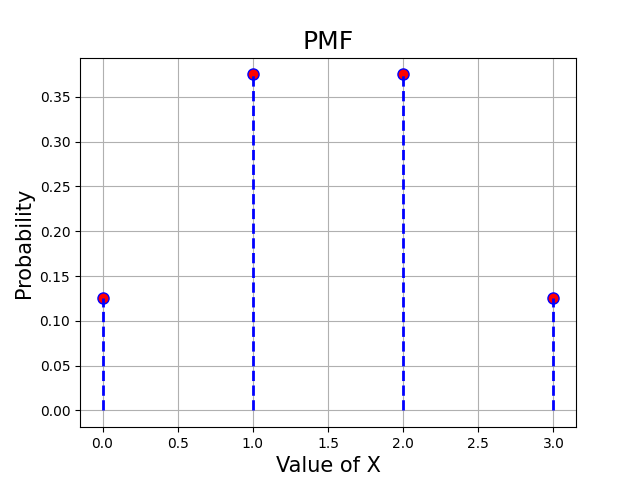
\includegraphics[width=\columnwidth]{prv4.png}
    \caption{Plot of the PMF}
    \label{fig:fig-1}
    \end{figure}

	\begin{align}
	   \fbox{$\pr{X = k} = \comb{n}{k}\brak{p}^k\brak{1-p}^{n-k}$} \label{3}
	\end{align}
	where $k= 0,1,\dots, n$ which is/are the number of Heads in the $n$ trials.
    	
   Now, Let the random variable $Z \in \cbrak{0,1}$ denotes the outcome of the game such that : 
    \begin{table}[ht!]
        \centering
        \def\ifundefined#1{\expandafter\ifx\csname#1\endcsname\relax}
\ifundefined{inputGnumericTable}
	\def\gnumericTableEnd{\end{document}}

	\documentclass[12pt%
			  %,landscape%
                    ]{report}
       \usepackage[latin1]{inputenc}
       \usepackage{fullpage}
       \usepackage{color}
       \usepackage{array}
       \usepackage{longtable}
       \usepackage{calc}
       \usepackage{multirow}
       \usepackage{hhline}
       \usepackage{ifthen}
       \usepackage[misc]{ifsym}
	\begin{document}
\else
    \def\gnumericTableEnd{}
\fi
\providecommand{\gnumericmathit}[1]{#1} 
\providecommand{\gnumericPB}[1]%
{\let\gnumericTemp=\\#1\let\\=\gnumericTemp\hspace{0pt}}
 \ifundefined{gnumericTableWidthDefined}
        \newlength{\gnumericTableWidth}
        \newlength{\gnumericTableWidthComplete}
        \newlength{\gnumericMultiRowLength}
        \global\def\gnumericTableWidthDefined{}
 \fi
 \ifthenelse{\isundefined{\languageshorthands}}{}{\languageshorthands{english}}                                                      %%
\providecommand\gnumbox{\makebox[0pt]}                       %%
\setlength{\bigstrutjot}{\jot}
\setlength{\extrarowheight}{\doublerulesep}
\setlongtables

\setlength\gnumericTableWidth{%
	50pt+%
	170pt+%
0pt}
\def\gumericNumCols{4}
\setlength\gnumericTableWidthComplete{\gnumericTableWidth+%
         \tabcolsep*\gumericNumCols*2+\arrayrulewidth*\gumericNumCols}
\ifthenelse{\lengthtest{\gnumericTableWidthComplete > \linewidth}}%
         {\def\gnumericScale{1*\ratio{\linewidth-%
                        \tabcolsep*\gumericNumCols*2-%
                        \arrayrulewidth*\gumericNumCols}%
{\gnumericTableWidth}}}%
{\def\gnumericScale{1}}


\ifthenelse{\isundefined{\gnumericColA}}{\newlength{\gnumericColA}}{}\settowidth{\gnumericColA}{\begin{tabular}{@{}p{50pt*\gnumericScale}@{}}x\end{tabular}}
\ifthenelse{\isundefined{\gnumericColB}}{\newlength{\gnumericColB}}{}\settowidth{\gnumericColB}{\begin{tabular}{@{}p{170pt*\gnumericScale}@{}}x\end{tabular}}

	\begin{center}
\begin{tabular}[c]{%
	b{\gnumericColA}%
	b{\gnumericColB}%
	}

	\hhline{|-|-~}
	 \multicolumn{1}{|p{\gnumericColA}|}%
	{\gnumericPB{\centering}\gnumbox{\textbf{Event}}}
	&\multicolumn{1}{p{\gnumericColB}|}%
	{\gnumericPB{\centering}\gnumbox{\textbf{Description}}}
\\
    \hhline{|--|~}
	 \multicolumn{1}{|p{\gnumericColA}|}%
	{\gnumericPB{\centering}\gnumbox{$X=0$}}
	&\multicolumn{1}{p{\gnumericColB}|}%
	{\gnumericPB{\centering}\gnumbox{Hanif losing the game}}
\\
    \hhline{|--|~}
	 \multicolumn{1}{|p{\gnumericColA}|}%
	{\gnumericPB{\centering}\gnumbox{$X=1$}}
	&\multicolumn{1}{p{\gnumericColB}|}%
	{\gnumericPB{\centering}\gnumbox{Hanif winning the game}}
\\
\hhline{|-|-|~}
\end{tabular}
	\end{center}
	
\ifthenelse{\isundefined{\languageshorthands}}{}{\languageshorthands{\languagename}}
\gnumericTableEnd

    	\caption{Description of Events}
    	\label{Tables:Table}
    \end{table}
    
    \note The above $2$ events are mutually exclusive and exhaustive. 
    \begin{align}
        \implies \pr{Z = 0} + \pr{Z = 1} \equals 1 \label{4}
    \end{align}
    
    Hence, Probability of Hanif winning the game i.e., all the $3$ tosses resulting in either \underline{$3$ Heads} or \underline{$3$ Tails} is:
    \begin{align}
        \pr{Z = 1} = \pr{X = 0} + \pr{X = 3}
    \end{align}
    From the equation- \ref{3},
    \begin{multline}
    \pr{Z = 1} = \comb{3}{0}\brak{0.5}^0\brak{0.5}^{3-0} +\\ \comb{3}{3}\brak{0.5}^3\brak{0.5}^{0}
    \end{multline}
    
    On calculating, we get,
    \begin{align}
     \label{7}    \pr{Z = 1} = \frac{1}{8} + \frac{1}{8} = \frac{1}{4}
    \end{align}
    
    \noindent From the equations- \ref{4} and \ref{7}, The probability of Hanif losing the game is:
    \begin{align}
        \pr{Z = 0} &= 1 - \pr{Z = 1} = 1- \frac{1}{4}\\
        \implies \pr{Z = 0} &= \frac{3}{4}
    \end{align}
    
    Hence, the probability that Hanif will lose the game is \underline{$0.75$} 
\end{document}
